\chapter{Turvallisuus\label{Turvallisuus}}


\begin{figure}
    \centering
    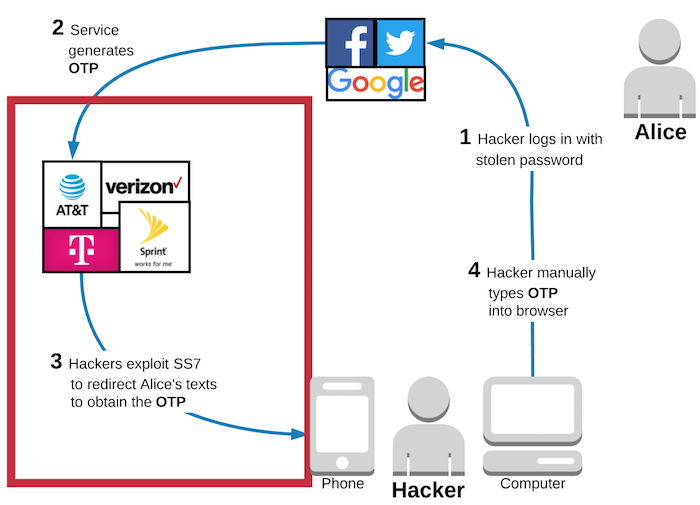
\includegraphics[width=10cm]{template/figures/SS7 attack vulnerable.png}
    \caption{SS7 haavoittuvuus SMS varmentamisessa}
    \label{fig:ss7SMSM}
\end{figure}

Kuvassa \ref{fig:ss7SMSM} havainnollistaa kaksivaiheisen kirjautumisen toimintaa, jossa käytetään salasanaa ja tekstiviestillä tulevaa vahvistuskoodia varmentamiseen. Ensimmäiseksi hyökkääjä kirjautuu varastetuilla tunnuksilla palveluun. Tämän jälkeen palvelu tunnistaa, että käyttäjällä on kaksivaiheinen tunnistautuminen käytössä. Palvelu luo kertakäyttöisen koodin ja lähettää sen tekstiviestinä. Tämän jälkeen siirrytään kuvan xx kolmanteen vaiheeseen, joka on merkitty punaisella kehyksellä. Kolmannessa vaiheessa hyökkääjä käyttää SS7 hyökkäystä kertakäyttöisen koodin saamiseksi. Tämän jälkeen hyökkääjä kirjoittaa kertakäyttöisen koodin ja hyökkääjällä on pääsy käyttäjätilille.